\chapter{Analysis}
Two environments are developed for comparing the \gls{drl} algorithms used in this thesis: \textbf{single-agent bilateral negotiation environment}(\gls{sbe}) and multi-agent \textbf{concurrent bilateral negotiation environment}(\gls{mcbe}). The details are described in section \ref{single-agent-env} and \ref{multi-agent-env}. In addition to these environments, some methods have been implemented to make the training logic clearer, such as \texttt{Game} in section \ref{game} and \texttt{Scenario} in section \ref{scenario}.

\section{\gls{negmas} with \gls{openai gym}}
\gls{negmas} has implemented some negotiation mechanisms and specific simulated world, such as \gls{saom} and \gls{scml}(now as an independent project). In order to compare the algorithms in a specific simulated world more easily, an interface is needed to connect \gls{negmas} and \gls{rl} algorithms. This interface and all algorithms can be rewritten from scratch, but it is very time-consuming and not ideal. The second option is to implement some interfaces of an existing RL framework, which will reduce the required work. OpenAI realizes the environmental standardization and comparison of algorithms with the help of toolkit \gls{openai gym}\parencite{brockman2016openai}. Although \gls{openai gym} is not enough to complete the work in this thesis, the baseline algorithms and the environmental interface in the package greatly speed up the work. In this section, the implementation of training environment and assisted methods used in bilateral negotiation will be presented.

With the help of \gls{openai gym}, a bilateral negotiation environment can be developed on top of \gls{saom} from \gls{negmas} to study reinforcement learning algorithms. The package \textbf{Stable Baseline} \ref{backgrounds:stable-baselines} implemented many baseline algorithms, which can be easily tested in a custom environment.

\subsection{Configuration}
\subsubsection{Negotiation Issues}
\gls{negmas} provoides some classes and methods to design issues flexibly. In \gls{sbe}, following issues are used:
 
\begin{itemize}
	\item \textbf{PRICE:} Integer between two values, such as (10, 20)
	\item \textbf{QUANTITY:} Integer between two values, such as (1, 10)
	\item \textbf{TIME:} Relative step between zero and maximal step.
\end{itemize}


In the section "Experiment" \ref{sbe:experiment} of Chapter "Methods and Experiments", the configuration of the training environment will be listed in detail.
 
\subsection{Model}
The model consists of five parts, \textbf{environment \gls{sbe}}, \textbf{negotiation game}, \textbf{negotiation mechanism}, \textbf{negotiator} and \textbf{\gls{rl} trainer}.
Except for the negotiation mechanism mentioned in sections \ref{autonomous-negotiation} and \ref{background:negmas}, others parts will be introduced step by step in the following sections. 

First, we give a brief introduction of the five parts in this section.
\textbf{Environment \gls{sbe}} inherits from \texttt{gym.env} and implements the interfaces, mainly the step function. 
\textbf{Negotiation Game} controls the logic and several properties of the negotiation(e.g. negotiaton issues, type of learning strategies)and provides the functions and parameters required by training algorithms.
\textbf{Negotiation Mechanism} is realized in the simulator \gls{negmas}.
\textbf{Negotiator} is a general class of negotiators, which can execute negotiation behavior and have learning ability in \gls{sbe}.
\textbf{Trainer} is the true learnable agent corresponding to the reinforcement learning algorithm, which receives observation, state from \gls{sbe}. After training and feedward calculation it sends the action to \gls{sbe}. Then, the interactive agent in the environment will execute this action. The entire model is shown in \ref{fig:environment-single-agent}.
\begin{figure}[htbp]
\centering
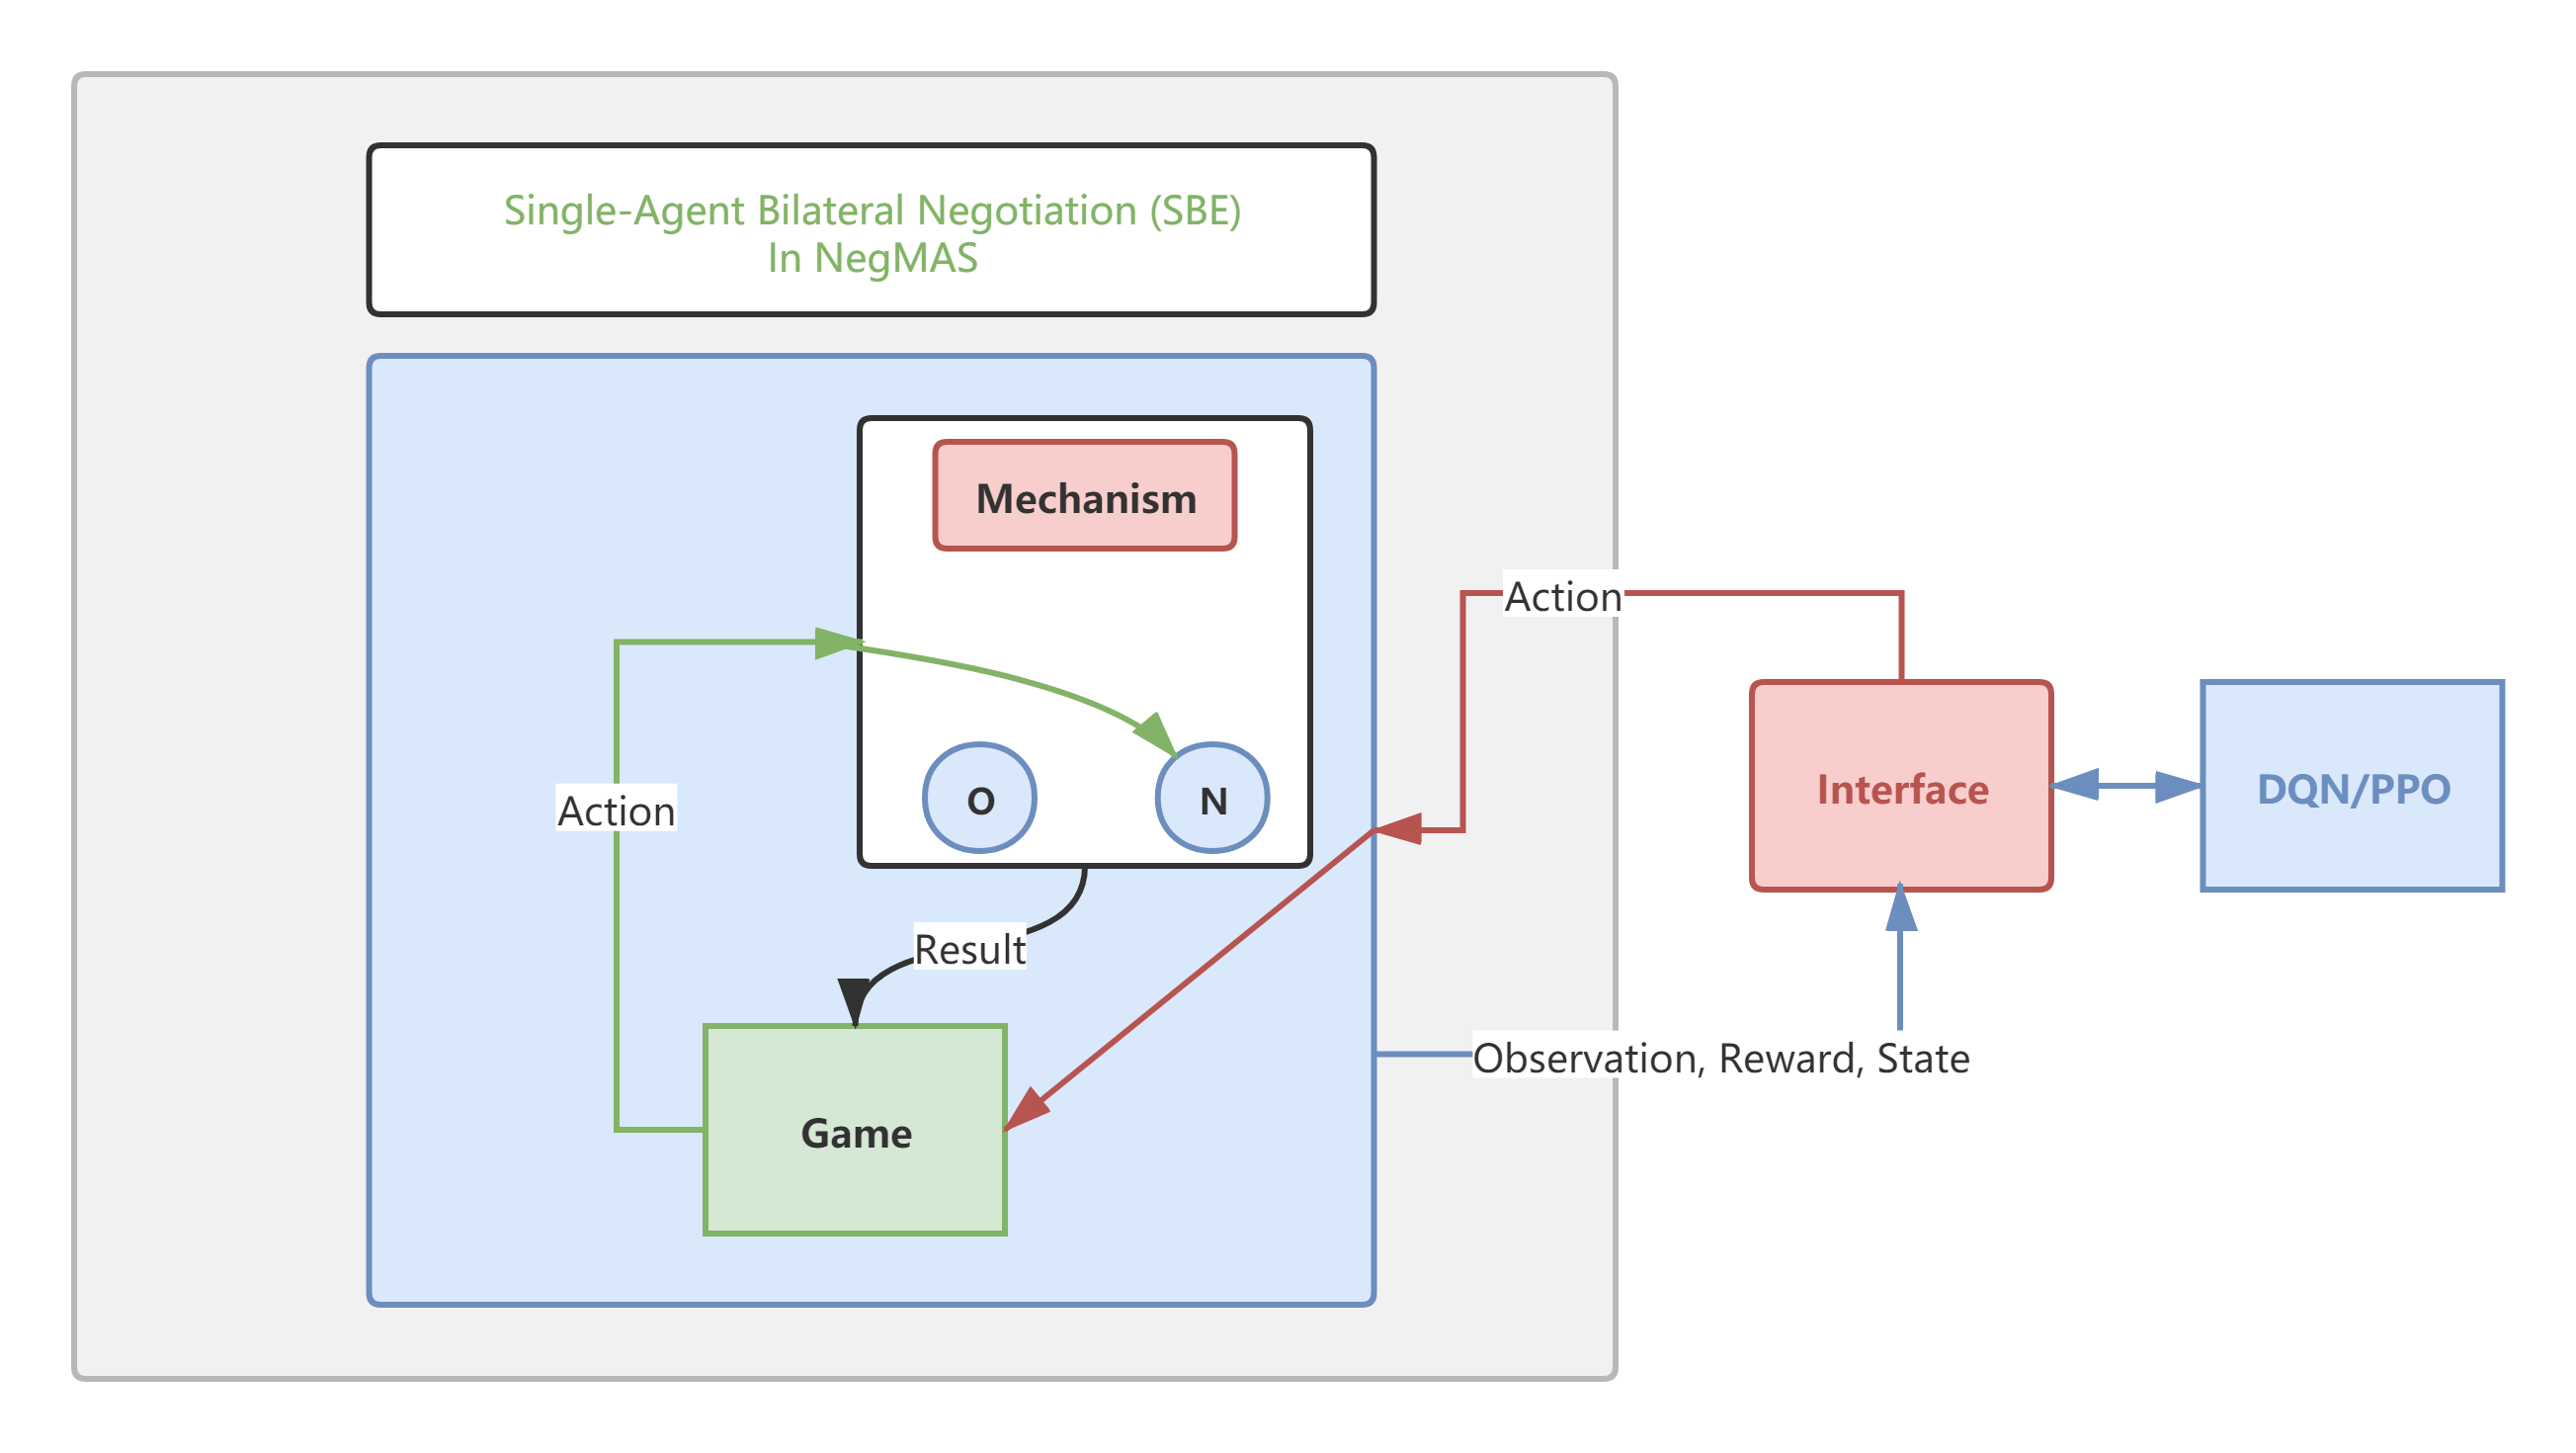
\includegraphics[width=0.80\textwidth]{./images/sbe.png}
\caption{Model for single agent bilateral negotiation based on NegMAS}
\label{fig:environment-single-agent}
\end{figure}

\subsection{Single-Agent Environment} \label{single-agent-env}
Since the default interface of the \gls{openai gym} environment was designed for single-agent as standard, we only need to examine how the \gls{sbe} can be represented via this interface and controlled by the controller. The interface methods of \gls{sbe} are therefore defined explicit below. 

\paragraph{STEP} First, sets up but does not perform the action received from trainer for the negotiator. Then, runs the negotiation mechanism, such as \gls{saom}, for one step. All actions will be performed by the negotiation mechanism. Finally, this function returns four parameters.

\begin{itemize}
	\item Observation: Offer proposed by opponent and current relative time.
	\item Reward: Utility value of the current offer and extra reward when an agreement is reached.
	\item Done: Reaches the final state or there is no agreement within the maximum running time.
	\item Info: State of the negotiation mechanism, extra info(i.e., state from negotiation mechanism(e.g, SAOMechanism)) used for evaluation.
\end{itemize}

\paragraph{RESET} resets the environment to an initial state and returns an initial observation, which contains negotiators' initial observation and other information relative to the design of the training environment. It will reset some environmental parameters at the same time, such as time and current step and creates a new negotiation mechanism session.
\paragraph{RENDER} This application is not required because there is no visual output.
\paragraph{CLOSE}  This application is not needed because there is no need to save the data created by the environment.
\paragraph{SEED} Sets the seed for the env's random number generator(s), such as random generator in negotiation mechanism.

\subsection{Game} \label{game}
In addition to implementing the official \gls{openai gym} \texttt{Env} interface, class \textbf{Game} is designed to control the entire negotiation mechanism. The purpose of this design is to reduce the modification of negotiatioin mechanism in \gls{negmas}. In this class, there are some parameters, which are received from the mechanism in \gls{negmas} and passed to the \gls{rl} algorithms as additional information(e.g., goal of learning). The two main methods are defined below.
 
\paragraph{STEP} Checks the state of \texttt{Game}, runs the negotiation mechanism for one step.
\paragraph{STEP\_FORWARD} realizes the key logic for the running of the negotiation mechanism, because negotiator can learn different strategies(acceptance and offer strategy) in \gls{sbe}. 

\subsection{Challenges of the environment}
Although \gls{openai gym} provides a unified interface for custom environments, it has some problems, which cannot be directly solved by the interface. These problems occurred during environmental design and will be listed and discussed in the following sections. 

\subsubsection{Design of Action Space and Observation Space}
One relevant consideration is related to \gls{rl} In \parencite{Bakker2019RLBOAAM}, the author study a modular \gls{rl} based on BOA (Bidding strategy, Opponent model and Acceptance condition) framwork which is an extension of the work done in \parencite{Bakker2019RLBOAAM}. This framework of \gls{rlboa} implements an agent that uses tabular Q-learning to learn the bidding strategy by discretizing the continuous state/action space (not an optimal solution for large state/action spaces as it may lead to curse of dimensionality and cause the loss of relevant information about the state/action domain structure too) \parencite{bagga2020deep}. 
Compared with tabular Q-learning, deep reinforcement learning algorithms use neural networks to solve this problem.
 
There are at least two possible approaches to implementing deep reinforcement learning for this learning case:

The first method: The output size of neural network is directly related to the size of the action space, in other words, it is equal to the size of the outcome space. 

The second method: Discrete action space is replaced by continuous action space. Before applying the action, filter invalid actions and scale valid actions.

The state in this experiment is opponent offer(PRICE, QUANTITY, TIME). When learning different strategies, the actions are different. For acceptance strategy, actions are $ACCEPT\_OFFER$, $REJECT\_OFFER$, $END_NEGOTIATION$ and $NO\_RESPONSE$. For offer strategy, actions are outcomes.

\subsubsection{Design of Reward Function}
The design of the reward function is the key point in the realization of \gls{rl} algorithm. This is very easy to understand, learners learn by evaluating the value of actions. Therefore, the reward function will directly affect the learning effect, and it is very necessary to design a good reward function. In \gls{sbe}, the utility function defined by \texttt{Negotiator} can be used as a calculation tool for obtaining the current offer reward, which can be intuitively set as part of the reward function. In order to encourage negotiators to sign the contract, an extra reward will be given when the contract is successfully signed. Hence, the reward function is defined as follows:
\begin{equation}
R_{t}=\left\{\begin{array}{ll}
1 - d(u(a), u(o)) + e & \text {accept offer}\\
1 - d(u(p), u(o))  & \text {reject, propose meaningful offer} \\
-1 & \text{otherwise}
\end{array}\right.
\end{equation}

Where $d(u(a), u(o))$ denotes the distance between of utility of an agreement and utility of optimal offer.  $d(u(p), u(o))$ denotes the distance between of utility of a proposal offer and utility of optimal offer. When at the last step, agent reachs an agreement, a extra reward (e) will be added into the reward.

\subsection{Analysis of the reinforcement learning algorithms}
\subsubsection{Policy-based vs. Value-based}
Policy-based(e.g., \gls{pg}, \gls{dpg} and \gls{ppo}) methods use a policy $\pi:s \to a$ to output action based on state and keep the parameters in the memory. Value-based(e.g., tabular q-learning, \gls{dqn} and \gls{sarsa}) methods do not explicitly store any policy, only a value function or value tabular. The policy can be implicitly derived from the value function(e.g., greedy selection). A well-known \gls{rl} framework A2C combined both policy-based and value-based parts.

\subsubsection{Model-based vs. Model-free}
One problem when applying the \gls{rl} is whenever you are in state $s$ and make an action $a$ you might not know the next state $s^{\prime}$.

For model-based approach learner has access to the model(i.e., environment or world) and knows some parameters, such as transition probability between states. Generally, if learner can predict the next state $s^{\prime}$ or reward $r$ after learning, these approaches of this learner are model-based. In model-free learner will collect some experience and derive optimal policy. It is not given any explicit information of model.

\subsection{Conclusion}
With the help of \gls{openai gym} and \gls{negmas}, the design of \gls{sbe} and the training of negotiators are not too complicated. The purpose of this part is to explore the implementation possibilities of deep reinforcement learning negotiators.

\section{\gls{scml} with \gls{openai gym}}
\subsection{Configuration}
\subsubsection{Negotiation Issues}
\paragraph{Standard \gls{scml}} Negotiation issues are multi-issues, Quantity, Time and Price. 
\paragraph{\gls{scml-oneshot}} Negotiation issues are multi-issues, Quantity and Price. Time is not important in this simulated world. All contracts will be executed at the same step in which agents reach agreements.

\subsection{Model}
The model consists of six parts: environment \texttt{\gls{mcbe}}, Scenario, World, Agent, Interfaces and \gls{madrl} algorithms(trainer).
All six parts are needed to be rewritten according to \gls{scml} and \gls{openai gym}. 
\textbf{Environment \texttt{\gls{mcbe}}} is a new universal environment for multi-agent learning. The key functions have the same names as functions in \gls{sbe}, such as \texttt{step}. It provides the pre-definition action spaces and observation spaces.  Additionally, the function \texttt{run} is used to run the complete simulation process. 
\textbf{Scenario} is the same as the class \texttt{Game} designed in \gls{sbe}. However, it does not consider the detailed logic of the game. The configuration of \gls{scm} world and the interactive logic of the agent with environment will be set and implemented by class scenario.
\textbf{World} is the key class which simulates the \gls{scm} world. Negotiation and manufacturing process are executed by it.
\textbf{Agent} is a general abstract class of agents(factory manager) which can run in \gls{mcbe}. 
\textbf{Interfaces} are a type of classes and functions, which control communication between environment and algorithms.
\textbf{\gls{madrl} algorithms(trainer)} are deep reinforcement learning algorithms(trainer) used for training multi-agent.
Entire model is shown in \ref{fig:environment-multi-agent}. Using \gls{madrl} algorithms can avoid the challenge of non-stationary environment and train multi-agent together to maximize the profit of the same type of agent.

\begin{figure}[htbp]
\centering
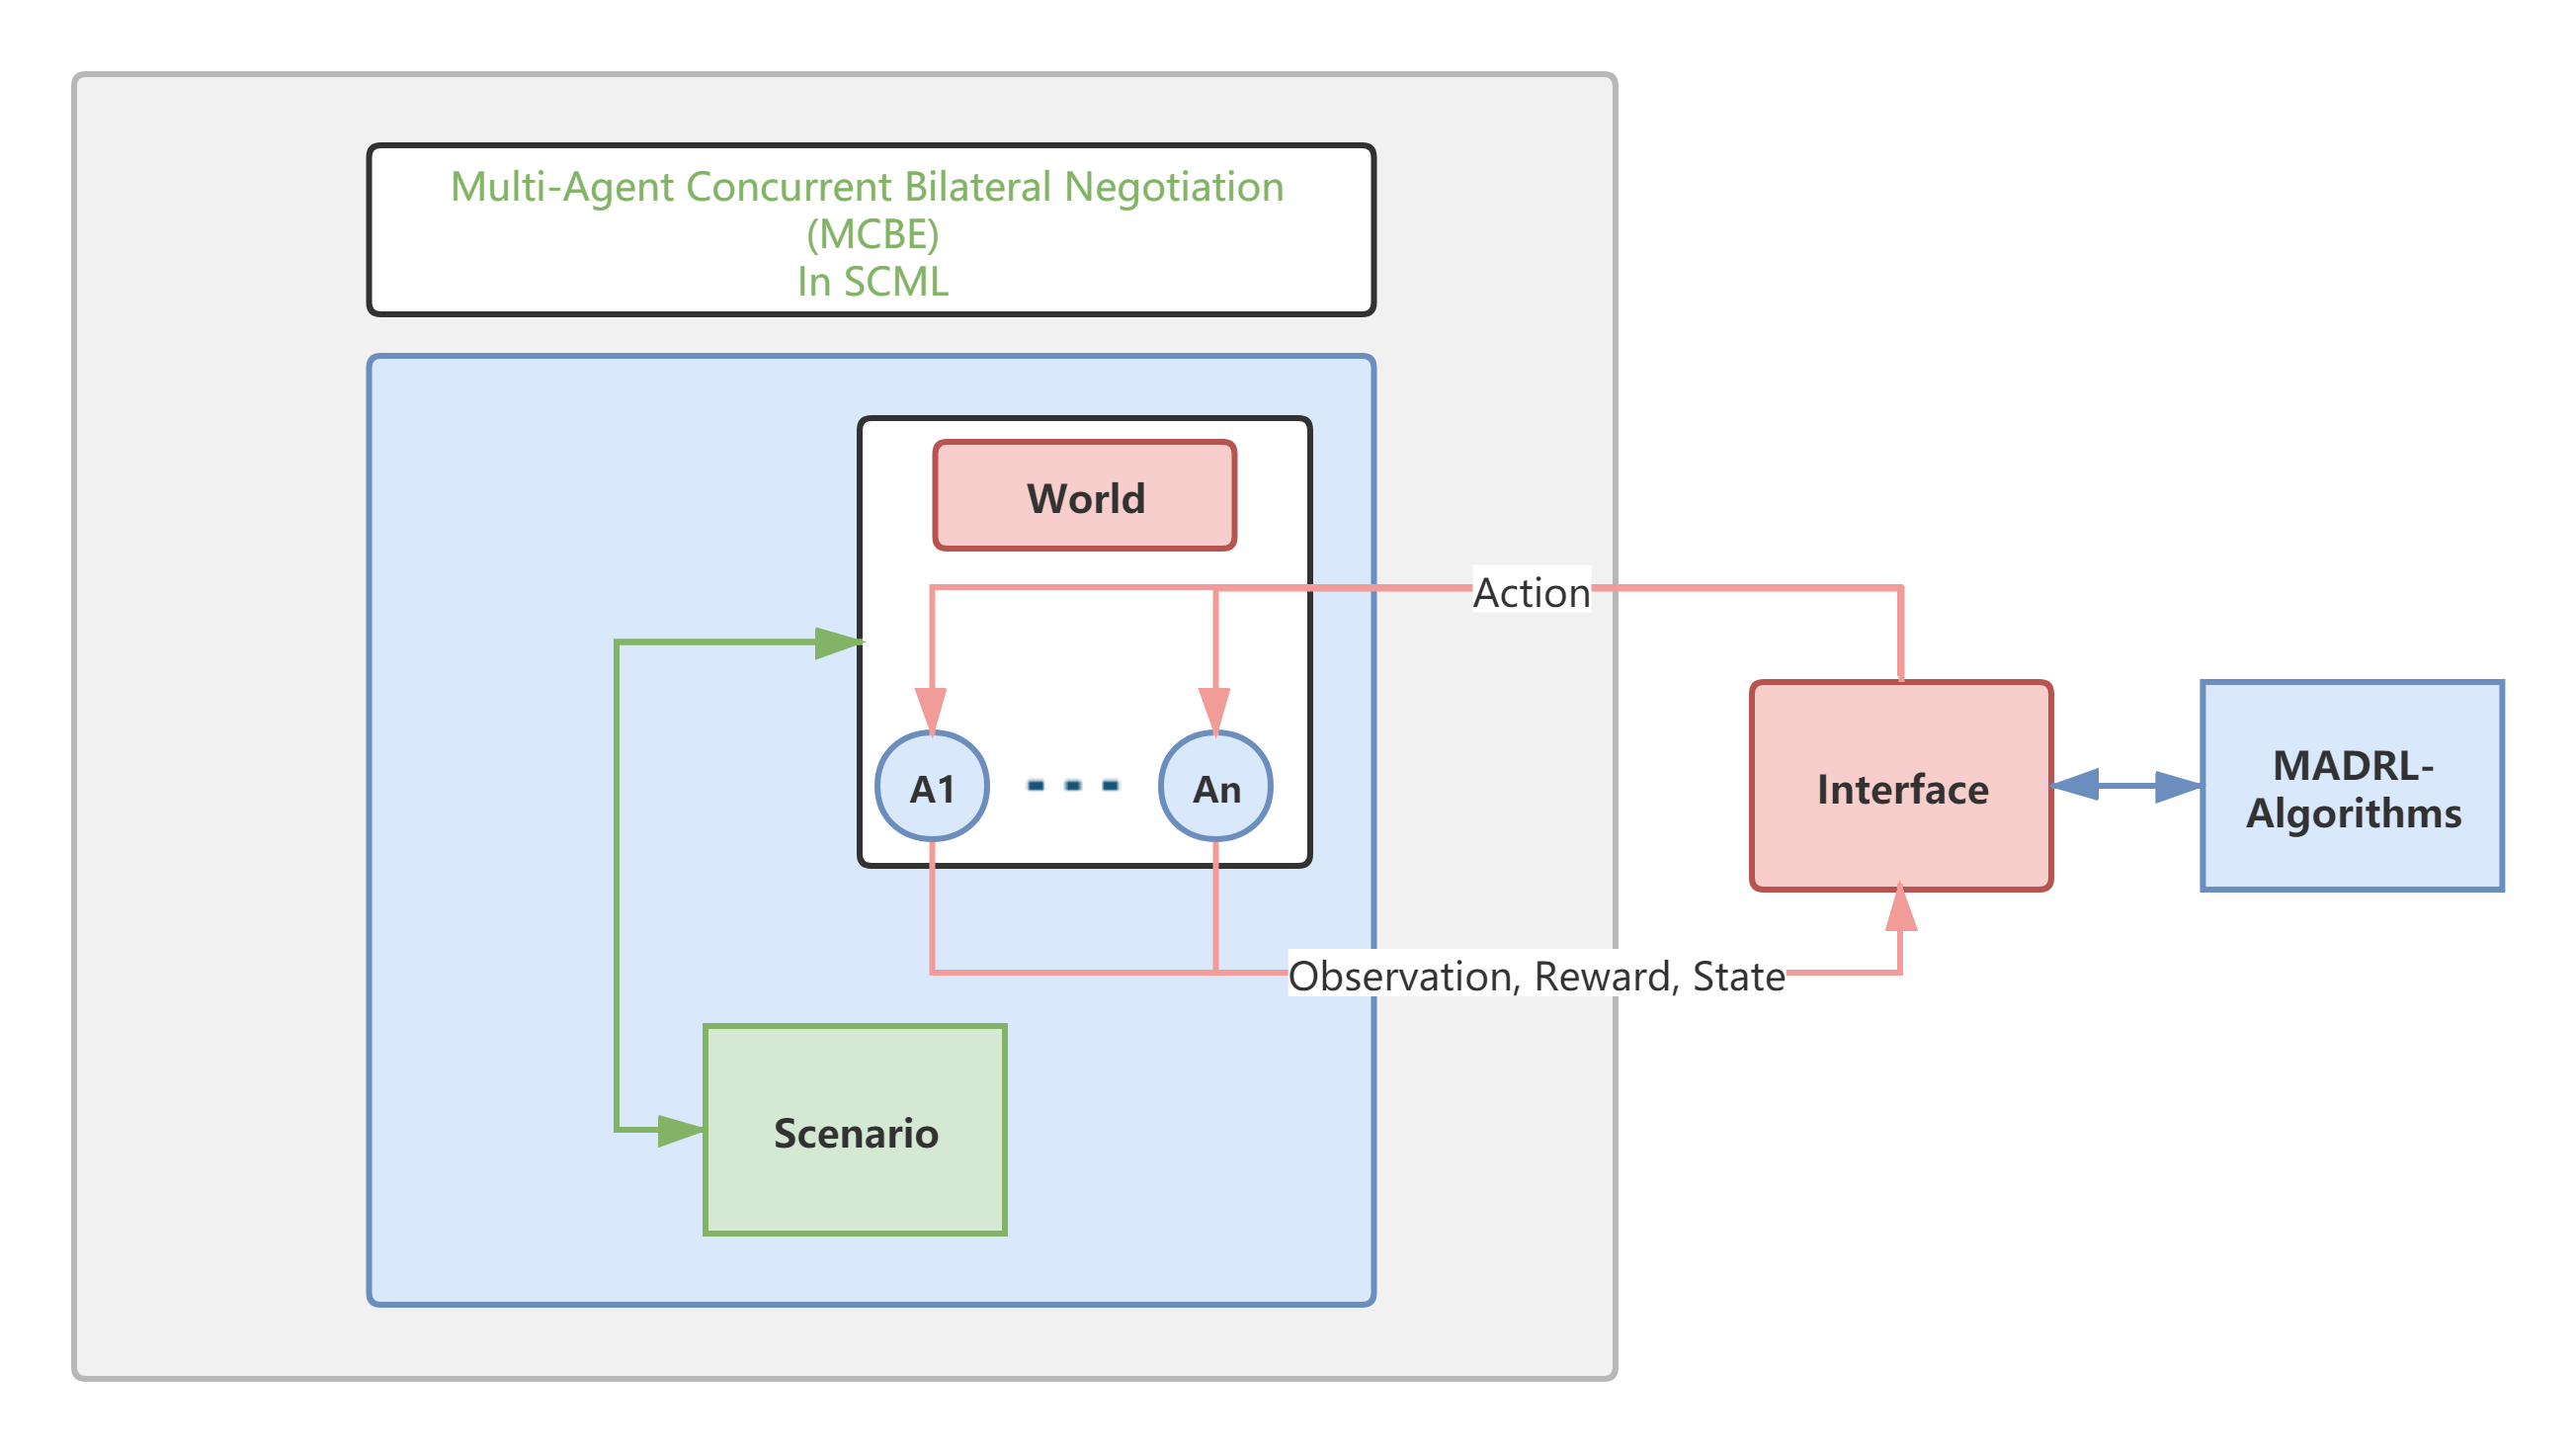
\includegraphics[width=0.9\textwidth]{./images/MCBE.png}
\caption{Model for Multi-Agent Concurrent Bilateral Negotiation based on \gls{scml}}
\label{fig:environment-multi-agent}
\end{figure}

\subsection{Multi-Agent Environment} \label{multi-agent-env}
In order to be able to realize deep reinforcement learning for multi-agent with an OpenAI Gym Environment, the interface would have to be expanded. In the following, alternative possibilities for using an OpenAI Gym Environment for \gls{marl} are discussed. 
In addition to implementing the \gls{openai gym} env interface methods, \gls{mcbe} added a new method called \texttt{run} to execute the entire episode.
\paragraph{STEP} Runs the simulated world for one step.
\paragraph{RESET} Resets the environment(MCBE) and other related parameters to an initial state after every episode and returns an initial observation.
\paragraph{RENDER} This application is not required because there is no visual output.
\paragraph{CLOSE} This application is not needed because there is no need to save the data created by
the environment.
\paragraph{SEED} Sets the seed for this env’s random number generator(s)
\paragraph{RUN} Runs entire episode. After a negotiation step, the rewards, observations, actions, etc. are stored in the memory buffer. 
\begin{itemize}
	\item Observation: Current offer in negotiation mechanism. The observations of all agents are combined in one list. Agent can only access to its local observation during decentralised execution.
	\item Reward: Sum reward of all learnable agents. Cumulative reward of a single agent (\ref{analysis:scml:design-of-reward-function}) is the sum of utility value of the current offer after one negotiation round, utility value of agent after one simulation step and profit of agent after the completed simulation.
	\item Done: Reaches the final state (last step of simulation world) or the maximum running time.
	\item State: State of environment. It can be replaced by \texttt{Observation}.
\end{itemize}

\subsection{Scenario} \label{scenario}
Scenario describes the structure of simulation world. It is similar as the assisted method \texttt{Game} in \gls{sbe} and provides functions for generating and resetting the world. With the help of \textbf{Scenario}, many scenarios can be created without changing of \gls{mcbe}. Figure \ref{fig:supply-chain-scenario-1} diagrams a simple scenario.

\begin{figure}[htbp]
\centering
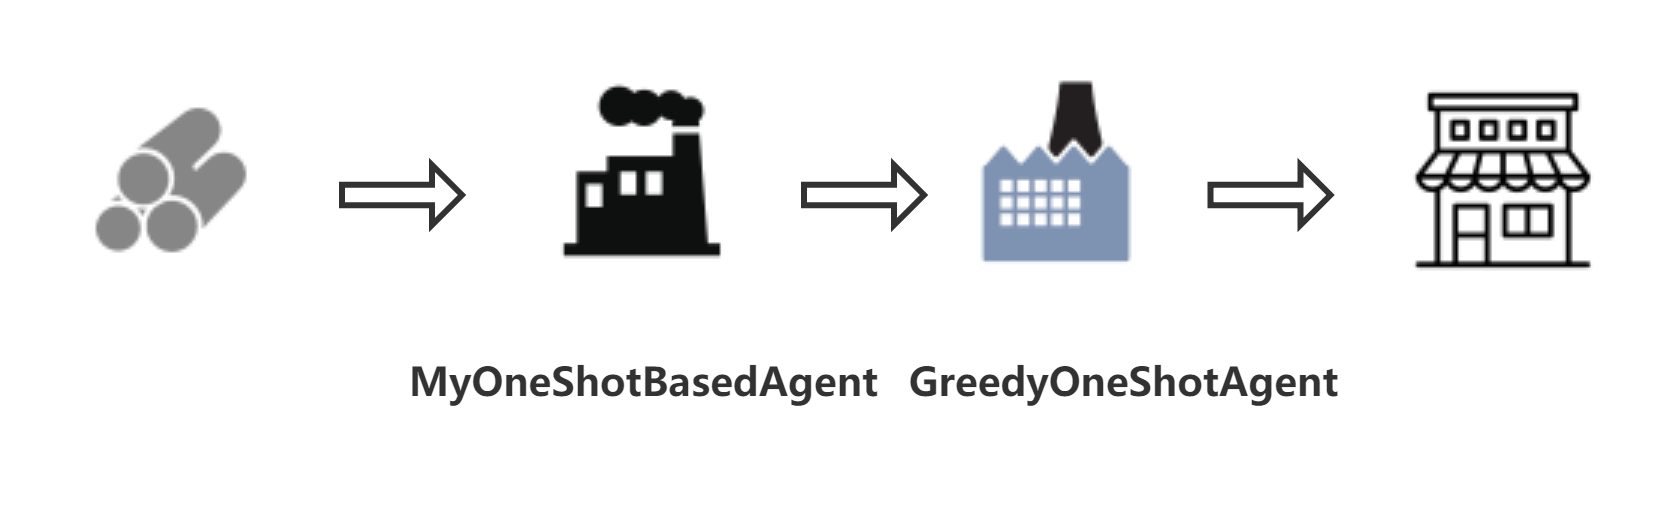
\includegraphics[width=0.9\textwidth]{./images/supply-chain-scenario-1.png}
\caption{Example of supply chain scenario, \gls{my-one-shot-drl-agent} vs. \gls{greedy-one-shot-agent}}
\label{fig:supply-chain-scenario-1}
\end{figure}

Interface of \textbf{Scenario}contains three normal functions and four callback functions passed to \gls{mcbe}.

\paragraph{MAKE\_WORLD} Creates instance of game or training world.
\paragraph{RESET\_WORLD} Sets the world to the initial state.
\paragraph{RESET\_AGENT} Resets agent, returns initial observation.
\paragraph{CALLBACK} OBSERVATION, REWARD, DONE and INFO

\subsection{Challenges of the environment}
\subsubsection{Combination with \gls{scml}}
Compared with \gls{sbe}, \gls{mcbe} can not directly call the functions designed in official \gls{scml}. \texttt{Step} in \gls{scml-oneshot} means one simulation step. In one simulation step, many negotiation rounds will be performed. The action of the agent is a \texttt{proposal}, so it needs to be meticulous to control every round of the negotiation mechanism in the simulation world. The class \texttt{TrainWorld} inherited from SCMLOneShotWorld achieves this goal.
\subsubsection{Design of Reward Function} \label{analysis:scml:design-of-reward-function}
In \gls{scm} world, the goal of the agent is to maximize profit at the end of the simulation. It is difficult to train an agent based on this reward signal alone. With the concept of reward shape \ref{related-work:sparse-reward} the reward signal can be split as three parts: utility value of current offer after every negotiation round, utility value of agent after every simulated step and profit at the end of simulation. The reward function of single agent $a_k$ is defined as follows:
\begin{equation}
R_{t}^{a_k}=\left\{\begin{array}{ll}
\sum_{j=0}^{N}\left({1-d_{n_j}(u(p), u(o))}\right) & \text {in negotiation}\\
u_{a_i}\left(C^{i}, C^{o}\right) & \text {end of one negotiation} \\
p_{a_k} & \text{end of simulation, profit}
\end{array}\right.
\end{equation}

Where, for negotiation $n_j$, $d_{n_j}(u(p), u(o))$ denotes the distance between utility of proposal offer($u(p)$) and utility of optimal offer($u(p)$). $N$ represents the maximum number of concurrent negotiations of the agent $a_k$. The utility function of agent ($u_{a}\left(C^{i}, C^{o}\right)$) is defined in the equation \ref{equation:utility-agent} from \parencite{Mohammad2021}. It represents the \textbf{expected profit} of a factory.

\begin{equation} \label{equation:utility-agent}
\begin{aligned}
u_{a}\left(C^{i}, C^{o}\right)=\sum_{c \in \bar{C}^{o}}\left(p_{c} q_{c}\right)-\sum_{c \in C^{i}}\left(p_{c} q_{c}\right)-m_{a} P_{a}-\gamma_{a} \mathrm{t} \mathrm{p}\left(p_{a}^{i}, s\right) Q_{a}^{i+}-\alpha_{a} \mathrm{tp}\left(p_{a}^{o}, s\right) Q_{a}^{o+}
\end{aligned}
\end{equation}
Where $C^{i}$ denotes the set of input contracts plus the exogenous input contracts. $C^{o}$ denotes the set of output contracts plus the exogenous output contracts. Price and quantity of the contract $c$ are formed by $p_c$ and $q_c$, respectively. Because the agent can only sell what it can produce, the set of satisfiable output contracts can be defined as $\bar{C}^{o}$. $Q^{i+}$ is simply the quantity to be bought  according to $C^{i}$ but is never sold. $p_{a}^{i}$ and $p_{a}^{o}$ are the input and output products, and $tp(p, s)$ is the current trading price of product $p$ at step $s$. The meaning of each term is listed below:
\begin{itemize}
\item \textbf{$\sum_{c \in \bar{C}^{o}}\left(p_{c} q_{c}\right)$} The total money it earns by selling its produced outputs.  
\item \textbf{$\sum_{c \in C^{i}}\left(p_{c} q_{c}\right)$} The total money it pays for buying its inputs.
\item \textbf{$m_{a} P_{a}$} The cost of producing the product.
\item \textbf{$\gamma_{a} \mathrm{t} \mathrm{p}\left(p_{a}^{i}, s\right) Q_{a}^{i+}$} The loss of buying too many inputs without using them immediately.
\item \textbf{$\alpha_{a} \mathrm{tp}\left(p_{a}^{o}, s\right) Q_{a}^{o+}$} The penalty for failed delivery of production products.
\end{itemize}

\subsection{Analysis of the reinforcement learning algorithms}
\subsubsection{Independent Learning vs. Centralized Learning}
\paragraph{Non-stationary environment}
Traditional reinforcement learning approaches such as Q-Learning or policy gradient
are poorly suited to multi-agent environments\parencite{maddpg2017, Rashid2018, en13010123}. One issue is that each agent’s policy is changing as training progresses, and the environment becomes non-stationary from the perspective of any individual agent (in a way that is not explainable by changes in the agent’s own policy).
Due to the non-stationary environment, a method called centralized learning and decentralized execution is proposed to train multi-agents.
\paragraph{Cooperative and Competitive} Independent learning agent consider just the goal of itself and can not deal with the cooperative and competitive problem. The centralized learning framework is an intuitive idea to solve this problem by changing the design of the reward function in different situations.

\subsubsection{\gls{maddpg} vs. \gls{qmix}}
Centralised learning of joint actions(\textbf{\gls{maddpg}}) can naturally handle coordination problems and avoids non-stationarity, but is hard to scale, as the joint action space grows exponentially with the number of agents. In \parencite{Rashid2018}, author proposed a neural network(\textbf{\gls{qmix}}) to transform the centralised state into the weights of another neural network. This second neural network is constrained to be monotonic with respect to its inputs by keeping its weights positive. This feature makes it possible to learn when there are many agents.

\subsection{Conclusion}
Compared with \gls{sbe}, \gls{mcbe} consider not just single learnable \gls{rl} agent. Multi-agent is the basic setting of this environment. Hence, the number of agent, the observation space and action space of single agent, the design reward are needed to be considered carefully. With the help of \gls{mcbe} developers just need to focus on the configuration of training scenario. \gls{mcbe} decouples well the algorithms and environment. 